\newpage
	\section{T} \label{sec:T}
	
		\subsection{TASK} \index{Task} \label{task}
		Cose da fare per arrivare a ciò che si vuole (diverso da compito e attività).
	
		\subsection{TECHNOLOGY BASELINE} \index{Technology Baseline} \label{technologybaseline}
		Dimostrare (a committente e a noi stessi) di disporre delle tecnologie, librerie e framework necessari per lo sviluppo del prodotto portando una baseline. Ne dimostra l'adeguatezza tramite \underline{\hyperref[poc]{Proof of Concept}}. È soggetta a verifica Agile. Collegato alla \underline{\hyperref[RP]{RP}}.
		
		\subsection{TEMPO/PERSONA} \index{Tempo/persona} \label{tempopersona}
		Quanto tempo produttivo sta usando quella persona(profilo). La sommatoria mi dà il costo complessivo.
		
		\subsection{TEST} \index{Test}	\label{test}	%7 dicembre - Verifica e validazione
		Prima di mettere insieme tutti i vari programmi in un prodotto SW, bisogna accertarsi che ogni piccola parte funzioni tramite test. %slide 5/22 set verifica e validazione
		Per questo conviene adottare la \textit{Continuous Integration} che è una metodologia intelligente. Essa mi fa scegliere prima i vari test che mi andranno a testare una parte di programma a cui ne manca ancora un'altra (esempio: l'interfaccia senza base dati). \\
		I principali test sono:
		\begin{itemize}
			\item \underline{\hyperref[testunita]{Test di unità}}
			\item \underline{\hyperref[testintegrazione]{Test d'integrazione}}
			\item \underline{\hyperref[testsistema]{Test di sistema}}
			\item Esistono anche \underline{\hyperref[testregressione]{test di regressione}} e test di accettazione (collaudo)
		\end{itemize}
		E devono essere 
		\begin{itemize}
			\item ripetibili: per questo si specifica ambiente di esecuzione, attese e procedure;
			\item automatizzati: per questo si usano strumenti come \textit{\underline{\hyperref[driver]{driver}}}, \textit{\underline{\hyperref[stub]{stub}}} e \textit{\underline{\hyperref[logger]{logger}}} (sono \underline{\hyperref[mock]{mock}});
			\item oggettivi e non personalizzati;
		\end{itemize}
		Ma fare i test in modo esaustivo è impossibile.
		\textbf{N.B:} tutte le regole dei test vengono decise nella progettazione.
		
		\begin{figure}[H]
			\centering
			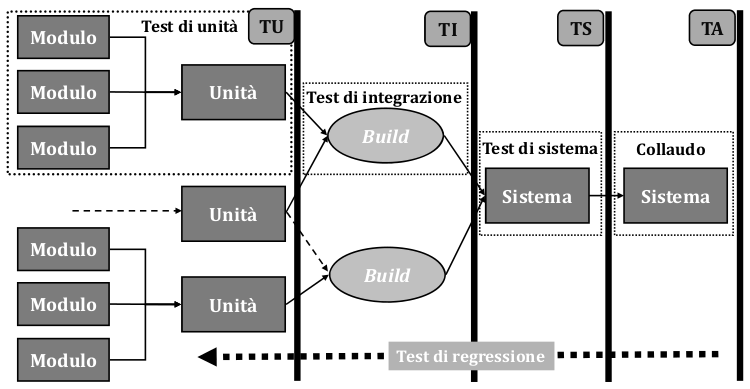
\includegraphics[width=0.9\textwidth]{img/test}		
			\caption{Tipi di test (analisi dinamica).}
		\end{figure} 
		%analisi dinamica % 20 dicembre
		I test comportano l'esecuzione dell'oggetto di verifica e devono dare misure di qualità. Ogni test deve avere un obiettivo:
		\begin{itemize}
			\item chiaro;
			\item utile;
			\item decidibile, perché c'è l'\underline{\hyperref[oracolo]{oracolo}}, ovvero deve produrre un esito verificato rispetto a un comportamento atteso;
		\end{itemize}	
		E il posto in cui dico queste cose è il \underline{\hyperref[pianoqualifica]{Piano di qualifica}}, perché lo dice il \underline{\hyperref[V]{modello a V}}. 
		
		Il verificatore controlla se ci sono problemi nei test. Se ci sono, essi sono dovuti a:
		\begin{enumerate}
			\item \underline{\hyperref[mistake]{mistake}};
			\item \underline{\hyperref[fault]{fault}};
			\item \underline{\hyperref[error]{error}};
			\item \underline{\hyperref[failure]{failure}}.
		\end{enumerate}
		Più obiettivi ha un test e peggio è. Più semplice è il SW da scrivere, più semplice sarà il test. La strategia richiede di trovare un bilanciamento tra la quantità minima e massima di casi di \underline{\hyperref[prova]{prova}} rispettando la legge del \underline{\hyperref[diminishingreturn]{rendimento decrescente}}.
		Secondo Bertrand Meyer: smantellare quello che ha in pancia un fault, ovvero bisogna sempre cercare di far fallire un test. \\ %..slide 13/34
		
		I test si specificano (\textit{Specifica}), poi (\textit{Codifica}) vanno tradotti in un eseguibile (da Codifica in poi voglio automatizzazione), collegati all'oggetto di test (\textit{Compilazione}), devo farli eseguire (\textit{Esecuzione}) e registrare l'esito (\textit{Analisi}). Infine l'output di un test si mette in un file chiamato file di log.
		
		\begin{figure}[H]
			\centering
			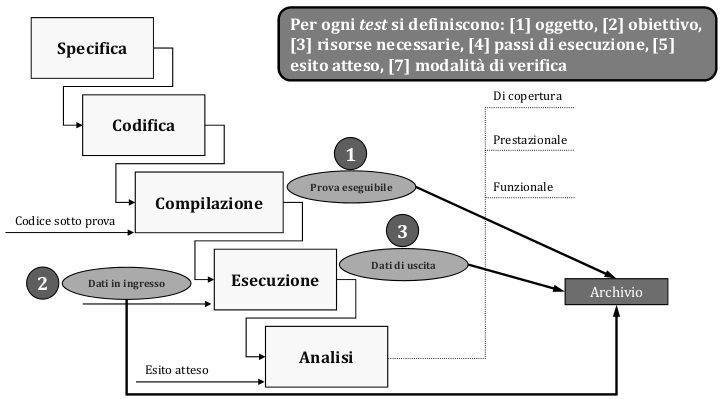
\includegraphics[width=0.8\textwidth]{img/prove}		
			\caption{Attività di prova.}
		\end{figure} 
		
		Si lavora per classi di equivalenza, in particolare 3: valori non ammessi, valori barriera, valori ammessi entro barriere. Ogni insieme ha un rappresentate nei test. È facile ordinare gli interi qua, dentro le classi di equivalenza, ma non altri valori come i numeri reali.
		
		Ci sono principalmente due tipi di test:
		\begin{itemize}
			\item \textbf{funzionale}: \textit{black-box} si occupa di vedere il tipo di uscita di quel test e credere che al suo interno vada tutto bene (ciascun insieme di dati di ingresso, campioni delle classi di equivalenza, che producono un dato comportamento funzionale costituisce un singolo caso di prova);
			\item \textbf{strutturale}: \textit{white-box} si occupa di cosa fa il test e non dell'effetto che produce, ricercando la massima copertura;
		\end{itemize}	
		Puntiamo ad avere massima copertura tramite i due \textit{coverage}.
		Due fattori di copertura: %slide 30/34
		\begin{itemize}
			\item \textbf{\underline{\hyperref[statementcoverage]{Statement Coverage}}};
			\item \textbf{\underline{\hyperref[branchcoverage]{Branch Coverage}}};
		\end{itemize}
		È difficile avere proprio il 100\%, quindi aver soddisfatto tutti i requisiti, anche se è il nostro obiettivo.
		\textbf{Attenzione}: i test vanno fatti, ma costano e questo non è banale.
			
		
		\subsection{TEST CASE}	\index{Test case}	\label{testcase}
		Una singola specifica di un singolo test. Case è un "insieme di" e specificatamente:
		\begin{itemize}
			\item ingresso;
			\item uscita;
			\item oggetto di prova;
			\item ambiente di sviluppo;
		\end{itemize}
	
		
		\subsection{TEST DI INTEGRAZIONE}	\index{Testi d'integrazione} \label{testintegrazione}
		Verifica il residuo, che non possiamo accettare da singolo, mettendo insieme due unità con una \textit{build}. Sono idealmente quindi parti indipendenti messe insieme per collaborare. L'integrazione, se c'è una buona architettura, è anche parallelizzabile. \\
		La logica di integrazione funzionale:
		\begin{enumerate}
			\item Seleziona le funzionalità da integrare;
			\item Identifica le componenti che svolgono quelle funzionalità;
			\item Ordina le componenti per numero di dipendenze crescenti;
			\item Esegue l'integrazione in quel determinato ordine.
		\end{enumerate}
		Più ne faccio, più piccola è la parte che sto testando. Il test di integrazione rileva problemi quali:
		\begin{itemize}
			\item errori residui nella realizzazione dei componenti;
			\item modifiche delle interfacce o cambiamenti nei requisiti;
			\item riuso di componenti dal comportamento oscuro o inadatto;
			\item integrazione con altre applicazioni non ben conosciute;
		\end{itemize}
		La strategia si basa sostanzialmente di proseguire per passi, aggiungendo "pezzi" fino al completamento. Adotta quindi una strategia incrementale. Assemblo prima i produttori e poi i consumatori, seguendo la mia architettura. Dovrebbe essere inoltre reversibile perché se, per esempio, assemblo A e B e questo non va bene, allora devo avere la possibilità di tornare indietro.
		Secondo gli approcci \underline{\hyperref[topdown]{top-down}} e \underline{\hyperref[bottomup]{bottom-up}} qui, più in alto ci sta l'interazione con l'utente, più in basso ci sta la persistenza. \\
		Scelgo bottom-up se l'utente non ha ancora un punto da cui lavorare. Si integrano prima le parti con maggiore utilità e minore dipendenza. Questa strategia riduce il numero di stub necessari al test ma ritarda la disponibilità di funzionalità di alto livello. \\
		Scelgo top-down se è utile negoziare con l'utente. Questa strategia comporta l’uso di molti stub ma integra a partire dalle funzionalità di più alto livello. %slide 26/34 
		Il test di integrazione ha tanti test quanti ne servono per accertarsi che tutti i dati scambiati attraverso ciascuna interfaccia siano conformi alla loro specifica e accertarsi che tutti i flussi di controllo previsti siano stati effettivamente provati.
	
		
		\subsection{TEST DI REGRESSIONE}	\index{Test di regressione}	\label{testregressione}
		Collegato fortemente agli altri test. È una ripetizione selettiva di \underline{\hyperref[testunita]{test di unità}}, \underline{\hyperref[testintegrazione]{test d'integrazione}} e \underline{\hyperref[testsistema]{test di sistema}}. Si assicura che una modifica fatta su un unità per correggere un problema, non faccia danno ad altre causando regressione. La regressione si riduce se il sistema è scarsamente accoppiato (per esempio tramite incapsulazione ecc). \\
		Torno indietro per correggere se qualcosa è andato male. Ma anche questo correggere può produrre errori. Con questo test dimostro che non torno indietro.
		
		
		\subsection{TEST DI SISTEMA}	\index{Test di sistema}	\label{testsistema}
		Se le componenti del programma sono buone, faccio il sistema. È per il fornitore e serve per dire che è tutto a posto controllando che tutti i requisiti siano soddisfatti (quindi per dimostrare la conformità del prodotto).	\\
		I test di sistemta hanno inizio quando è completato il \underline{\hyperref[testintegrazione]{test d'integrazione}} e sono per definizione a scatola chiusa, nera. È una \textit{self-fullfilling-prophecy}: non ho ansia, sono sicuro. Il test di sistema viene fatto quando faccio i requisiti (e ciò mi fa capire che non ci piacciono requisiti grandi, ma sminuzzati).
	
	
		\subsection{TEST DI UNITÀ}	\index{Test di unità}	\label{testunita}
		Problema che non so individuare l'\underline{\hyperref[unita]{unità}}. L'unità si sceglie quando si progetta. La \textit{liability} di ogni persona vogliamo che sia piccola in modo che l'unità sia facilmente verificabile e ragionevole. Se un'unità quindi non è determinata da un linguaggio di programmazione, sarà un aggregato di cose che noi chiamiamo \underline{\hyperref[moduli]{moduli}}.	\\
		Il test di unità segna il primo \textit{gate} e si svolge con il massimo grado di parallelismo.
				
		
		\subsection{TEST SUITE}	\index{Test suite}	\label{testsuite}
		Suite è un completo, per cui questo è un insieme di \underline{\hyperref[testcase]{test case}}, ma completo.
				
		
		\subsection{TOP-DOWN}	\index{Top-down} \label{topdown}
		Proseguire dal tutto alle parti. Fondamentalmente è un'esplorazione funzionale, senza preconcetti.
		
	
		\subsection{TRACCIAMENTO} \index{Tracciamento} \label{tracciamento}
		Si occupa della gestione dell'evoluzione dei \underline{\hyperref[requirements]{requisiti}}, motivo per cui è essenziale sapere sempre a che punto si è nella copertura(=soddisfacimento) dei requisiti. Il tracciamento dei requisiti è essenziale per il controllo sistematico di conformità. Mi dà le risposte alle domande:"\textit{Ho tutto o no? Ho cose superflue?}". Ogni parte del documento dell'Analisi dei Requisiti c'è per bisogni impliciti o espliciti (tipo dal capitolato d'assalto), quindi il tracciamento tiene conto di tutti i collegamenti.
		
		\begin{figure}[H]
			\centering
			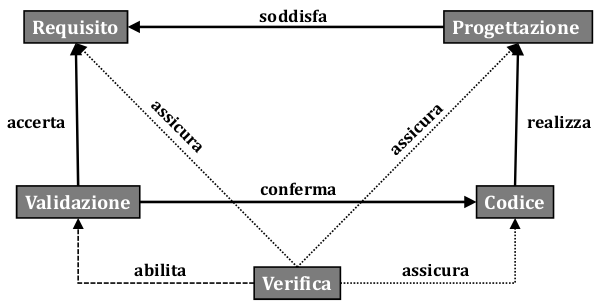
\includegraphics[width=0.7\textwidth]{img/trac}		
			\caption{Visualizzazione ordine del tracciamento dei requisiti.}
		\end{figure} 
	
		\textbf{Tracciamento sul codice}: \\ %slide 14/30	  13 dicembre - verifica e validazione: analisi statica
		Il tracciamento è qui vitale perché devo essere sicura di quello che sto facendo e di non fare cose oziose. Dimostra completezza ed economicità della soluzione e connette sempre parti correlate, infatti ha luoghi su ogni passaggio dello sviluppo (ramo discendente della \underline{\hyperref[V]{figura a V}}) e su ogni passaggio della verifica (ramo ascendente). Può essere altamente automatizzato.
		Particolari stili di programmazione facilitano il tracciamento, per esempio: assegnare singoli requisiti elementari a singoli moduli del programma richiede una sola procedura di prova (questo semplifica anche la verifica).
		
	
